\section{Extended Kalman Filter}

We now consider a scenario where the position is not measured directly. Instead, a distance sensor measures the Euclidean distance from the cart to a fixed point on a wall located at a horizontal offset \( d \) and vertical height \( h \) above the cart's equilibrium position. 

\begin{align}
    g(\mathbf{x}_k) = \sqrt{(r_k + d)^2 + h^2}
\end{align}

Since the measurement model is nonlinear, we use an Extended Kalman Filter (EKF) to linearize the measurement model around the predicted state at each time step.

\clearpage

\subsection{System Model and Linearization}

The process model remains unchanged since acceleration is still measured directly:

\begin{align}
    \mathbf{x}_k &= A_{k-1} \, \mathbf{x}_{k-1} + B_{k-1} \, a_{k-1} + \mathbf{w}_{k-1}, \quad \mathbf{w}_{k-1} \sim \mathcal{N}(0, Q_{k-1})
\end{align}

However, the measurement model changes due to the new sensor. 

\begin{align}
    y_k &= g(\mathbf{x}_k) + v_k, \quad\quad
    v_k \sim \mathcal{N}(0, R_k) 
\end{align}

The Jacobian \( C_k \) of the nonlinear measurement model at each time step is:


\begin{align}
    C_k = \frac{\partial g}{\partial \mathbf{x}} |_{\hat{\mathbf{x}}_{k|k-1}} =
    \begin{bmatrix}
        \dfrac{\hat{r}_{k|k-1} + d}{\sqrt{(\hat{r}_{k|k-1} + d)^2 + h^2}} & 0
    \end{bmatrix}
\end{align}

This Jacobian captures the sensitivity of the measurement to the state and is used in the EKF to compute the Kalman gain and update the estimate.

\subsection{Algorithm}

\textbf{Step 1: Initialization}

The initial state estimate \( \hat{\mathbf{x}}_0 \) is typically set to the expected 
initial position and velocity, i.e., \( \hat{\mathbf{x}}_0 = \mathbb{E}[\mathbf{x}_0] \). 
The initial state covariance \( P_0 \) represents the uncertainty in the initial estimate.

\begin{align}
    \hat{\mathbf{x}}_0 &= \mathbb{E}[\mathbf{x}_0] \\
    P_0 &= \mathbb{E}[(\mathbf{x}_0 - \hat{\mathbf{x}}_0)(\mathbf{x}_0 - \hat{\mathbf{x}}_0)^T]
\end{align}

\textbf{Step 2: Prediction Step}

In the prediction step, the state is predicted using the previous state 
estimate and the measured acceleration \( a_k \):

\begin{align}
    \mathbf{x}_{k|k-1} &= A \mathbf{x}_{k-1|k-1} + B a_k \\
    P_{k|k-1} &= A P_{k-1|k-1} A^T + Q
\end{align}

\clearpage

\textbf{Step 3: Update Step}


In the update step, the state estimate is corrected using the nonlinear measurement model. To apply the EKF, we linearize this measurement function. The Jacobian matrix \( C \) is computed as the derivative of \( g(\mathbf{x}) \) with respect to the state vector \( \mathbf{x} \):

\begin{align}
    C &= \frac{\partial g(\mathbf{x})}{\partial \mathbf{x}} \\
    S_k &= C P_{k|k-1} C^T + R \\
    K_k &= P_{k|k-1} C^T S_k^{-1} \\
    \mathbf{x}_{k|k} &= \mathbf{x}_{k|k-1} + K_k \left( y_k - g(\mathbf{x}_{k|k-1}) \right) \\
    P_{k|k} &= (I - K_k C) P_{k|k-1} (I - K_k C)^T + K_k R K_k^T
\end{align}

\subsection{Simulation Results}

The simulation uses the same system parameters as in the standard Kalman filter case. Regarding the distance measurement, the wall is located at a distance \( d = 5 \, \text{m} \) from the equilibrium position of the cart and at a height \( h = 5 \, \text{m} \).

Figure~\ref{fig:ekf} below shows the performance of the Extended Kalman Filter (EKF) when the position of the cart is not directly measured. The EKF is able to estimate both position and velocity accurately despite the nonlinear observation model. As shown in the plots, the filter effectively tracks the true position and velocity of the mass-spring-damper system. The estimation errors remain within the \( \pm 3\sigma \) confidence bounds, indicating that the EKF is well-tuned and the uncertainty estimates are consistent with the actual errors.

\begin{figure}[H]
    \centering
    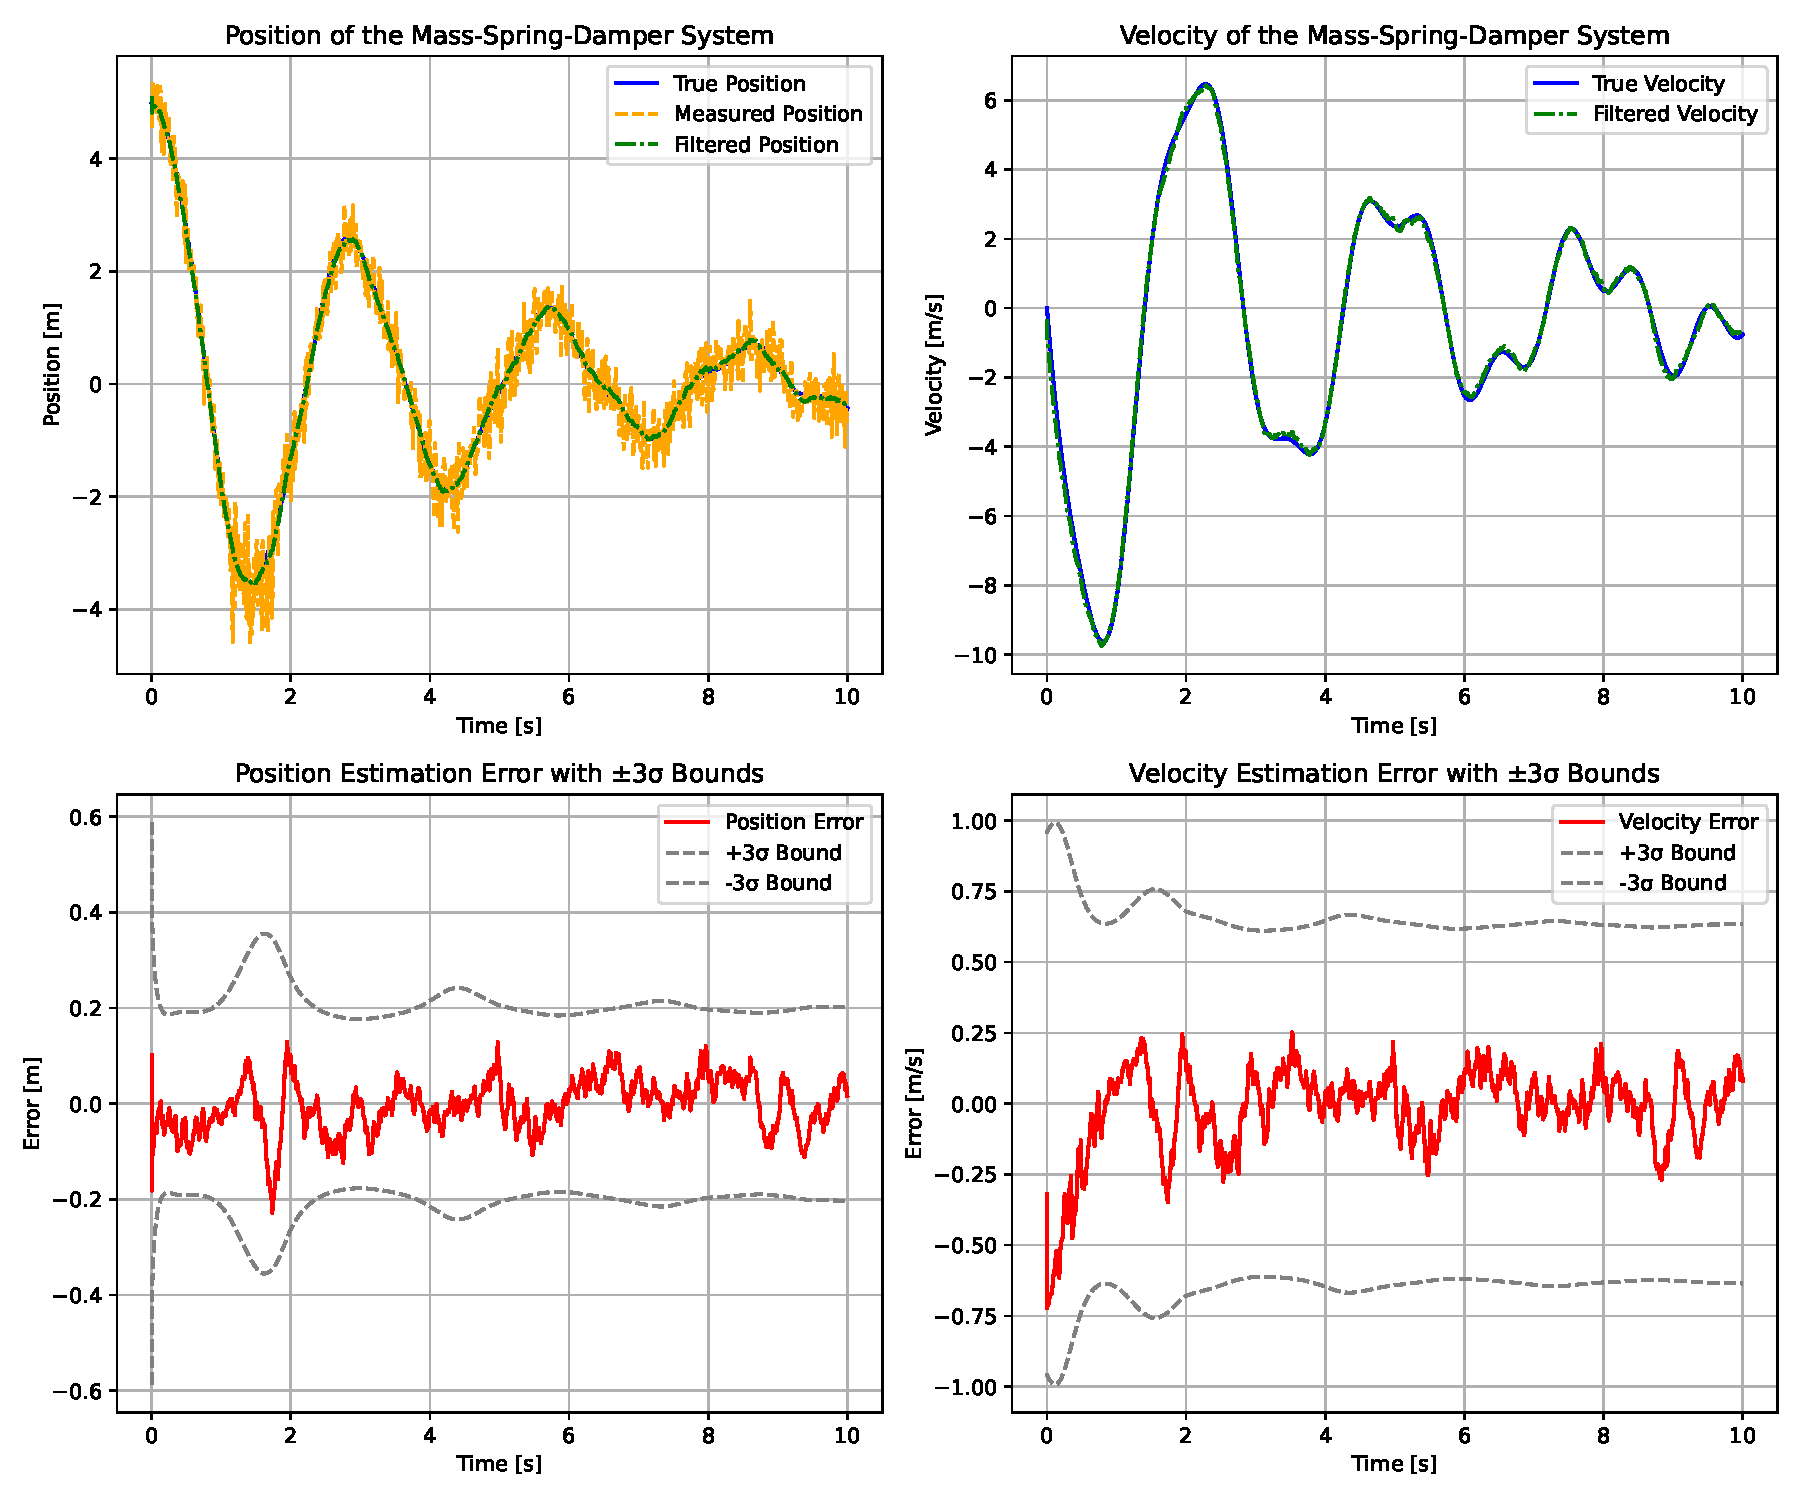
\includegraphics[width=1\textwidth]{figures/ekf.pdf}
    \caption{Extended Kalman filter estimation where the measurement is the Euclidean distance to a fixed point on the wall. The plots show the true, estimated, and measured values along with the estimation errors and \( \pm 3\sigma \) bounds.}
    \label{fig:ekf}
\end{figure}



